\documentclass[8pt]{beamer}
\usetheme{Copenhagen}
\usecolortheme{beaver}

\setbeamertemplate{navigation symbols}{}
\setbeamertemplate{headline}{}
\setbeamercovered{transparent=.5}

\usepackage{graphicx}
\usepackage{listings}
\usepackage{xcolor}

\newcommand{\code}[1]{{\small \texttt{#1}}}

% General document information
\author{
    \textbf{Student: Sepehr Mousavi} \\
    Teacher: Pablo Antolin Sanches
}
\title[Parallelization of the N-Body problem]{Parallel and GPU-accelerated algorithms for the N-body problem}
\subtitle[P-HPC]{MATH-454 Parallel and High-Performance Computing}
\institute[EPFL]{{École Polytechnique Fédérale de Lausanne}}
\date{\today}

\begin{document}

\frame{\titlepage}

\begin{frame}{Strong scaling of the parallel Barnes-Hut method}

    \begin{figure}
        \centering
        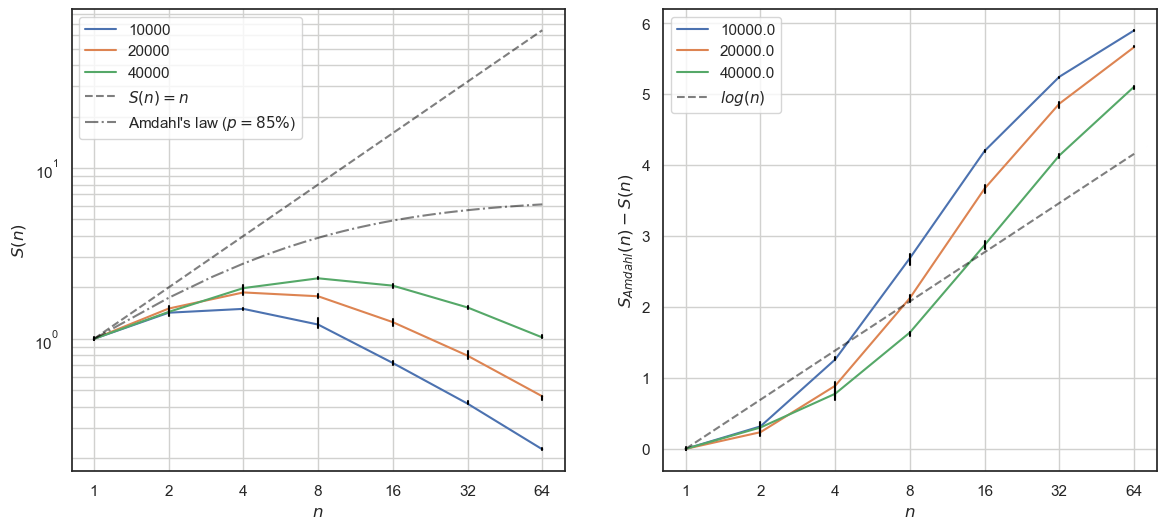
\includegraphics[width=.8\textwidth]{img/strongscaling.png}
    \end{figure}

    \begin{itemize}
        \item Parallelizable part of the code $\sim 85\%$ - {\small computing forces and movements}
        \item Even Amdahl's upper bound is limited - {\small maximum speed-up of 6 with 64 processors}
        \item Computational complexity $O(\frac{N}{n} \log N)$ - {\small because each process handles $\frac{N}{n}$ particles}
        \item Communication complexity $O(n \times \frac{N}{n} \log n)$ - {\small \code{MPI\_Ibcast} from each processor}
        \item Communication cost dominates the computational benefits with more processors
        \item The domination of communication cost happens later for larger problems
        \item The discrepency behaves as $O(\log n)$ - {\small same as communication with fixed $N$}
    \end{itemize}

\end{frame}

\begin{frame}{Weak scaling of the parallel Barnes-Hut method}

    \begin{figure}
        \centering
        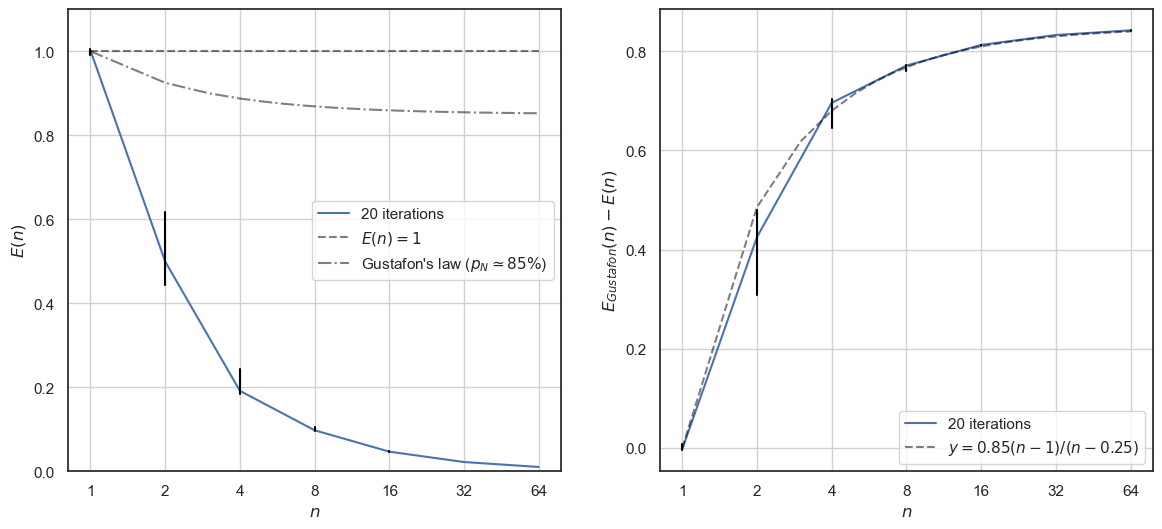
\includegraphics[width=.8\textwidth]{img/weakscaling.png}
    \end{figure}

    \begin{itemize}
        \item $p(N) \simeq 0.85$ is viable - {\small Construction of the tree (serial) has the same complexity}
        \item Huge discrepency from Gustafon's law - {\small the theoory does not count for communication}
        \item Constant computational work
            \\ \hspace{.25\textwidth} $W(n) = O(\frac{N}{n} \log N) = O(1) = W$
        \item We can replace $O(N \log N)$ with $O(n)$
        \item Communication cost
            \\ \hspace{.05\textwidth} $C(n) = O(N \log n) = O(N [\log N + \log(\log N)]) = O(N \log N) = O(n)$
        \item Efficiency $E(n) = \frac{T(1)}{T(n)} = \frac{W}{W + C(n)} = 1 - \frac{C(n)}{W + C(n)}$
    \end{itemize}

\end{frame}

\begin{frame}{Block sizes of the GPU-accelerated particle-particle method}

    \begin{columns}
        \column{.6\textwidth} {
            \centering
            \begin{itemize}
                \item Each thread handles one particle
                    \\ - {\small Last block with idle threads}
                \item Index is {\small \texttt{blockIdx.x * blockDim.x + threadIdx.x}}
                \item \texttt{cudaDeviceSynchronize}
                    \\ - {\small Before updateing the positions}
                    \\ - {\small After each iteration}
                \item Poor performance with 1 thread per block
                    \\ - {\small Only 1 active thread in each warp}
                \item Stagnates between 32 to 512 threads per block
                    \\ - {\small Warps are full and all SM's are used}
                \item Slight increase with 1024 threads per block
                    \\ - {\small Only 40 SM's are used}
                \item Not suitable for small problems
                    \\ - {\small Keeping the balance might be problematic}
                \item Better than the parallelized Barnes-Hut
                    \\ - {\small Only 0.53s compared to 0.89s with 8 processors}
            \end{itemize}
        }
        \column{.4\textwidth} {
            \centering
            \begin{figure}
                \centering
                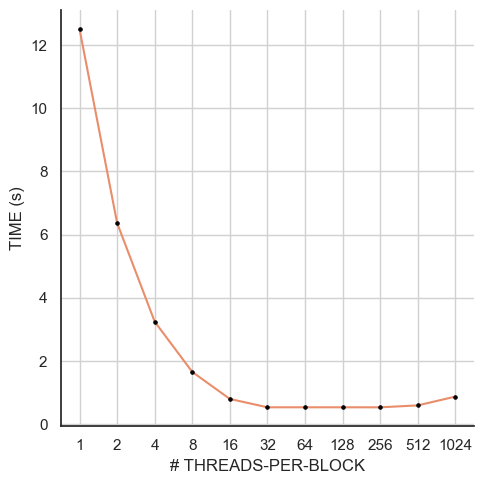
\includegraphics[width=\textwidth]{img/threadsperblock.png}
            \end{figure}
        }
    \end{columns}


\end{frame}

\end{document}
